% !TeX program = PdfLaTeX
% !TeX root = ../../Elaborati_Aerodinamica_Bruno_Spoti.tex
\chapter{Generalità e geometria del profilo alare PW106}

Il seguente lavoro si prefigge lo scopo di studiare le prestazioni aerodinamiche del profilo alare \emph{PW106}, un profilo disegnato da Peter Wick e ottenuto a partire dal profilo alare simile PW51 rispetto al quale ha una curvatura maggiore e quindi un maggiore $C_{l_\mathrm{max}}$. 
La valutazione delle caratteristiche dello stesso è stata condotta attraverso l'applicazione di metodi teorici tramite il codice XFOIL e con l'ausilio di script implementati in MATLAB.\\
Preliminarmente è stata trattata la geometria del profilo, la cui costruzione è stata fatta per punti. In seguito sono state ricavate le caratteristiche geometriche dello stesso e i risultati del profilo sottile. È stata poi studiata la soluzione in campo Euleriano incomprimibile a vari $C_l$ significativi, graficandone il coefficiente di pressione. Si è passati, poi, alla soluzione in campo viscoso introducendo gli effetti del numero di Reynolds e della turbolenza asintotica. Sono stati inoltre valutati gli effetti sullo strato limite in condizioni di alta portanza verificando, in base ai criteri semiempirici, il tipo di stallo del profilo in esame. Infine é stata ricavata l'aerodinamica del profilo considerando la deflessione di parte dello stesso come {\itshape flap} oppure come alettone.

\section{Geometria del Profilo}

La geometria del profilo è stata inizialmente fornita in forma tabellare con 33 punti sul dorso e 128 sul ventre riportata in figura~\ref{fig:puntiprofilo}. \cite{prof:sito} \\
Il profilo alare è stato fornito aperto al bordo d'uscita, e, prima di procedere con le analisi, sebbene il \emph{software} XFOIL sia comunque in grado di eseguire analisi su profili aperti, si è provveduto alla chiusura dello stesso tramite il comando {\itshape tgap}. Il confronto tra le due geometrie è riportato in figura~\vref{fig:BordoUscitaAperto}, mentre nella figura~\vref{fig:deltaz} sono riportate le differenze adimensionalizzate rispetto  alla corda tra le ordinate del profilo chiuso e quelle della geometria aperta.

L'operazione di chiusura del bordo d'uscita mostrata in figura~\vref{fig:BordoUscitaAperto} è stata fatta immettendo in XFOIL una distanza di fusione $d_f$ (\emph{blending distance}) unitaria. In questo modo, dall'analisi della differenza tra le ordinate del profilo aperto e quelle del profilo chiuso riportata in figura~\vref{fig:deltaz}, si nota che XFOIL esegue la chiusura atraverso uno \emph{scaling} delle ordinate lineare rispetto all'ascissa adimensionale.

Successivamente si è analizzato il modo in cui XFOIL chiude il profilo al variare della distanza di fusione $d_f$ tra 0 e 1 ottenendo le curve riportate in figura~\vref{fig:deltazdf}.

In particolare si nota come per $d_f=0$ vengono scalate solo le ordinate degli ultimi punti di dorso e ventre ottendendo il risultato riportato in figura~\vref{fig:confrontoApertoChiusodf0}.\\

Fatte queste osservazioni sui modi in cui XFOIL può chiudere il bordo d'uscita di un profilo si precisa che la designazione tecnica del profilo e le successive applicazioni sono state eseguite su una geometria ottenuta a partire da quella chiusa con $d_f=1$ sulla quale è stata effettuata un'interpolazione di tipo {\itshape Spline}, così da avere 100 punti sul dorso e 100 punti sul ventre, alle stesse ascisse. 
 
La scelta di migliorare la geometria del profilo fornita è stata fatta a causa della forte oscillazione nel grafico della curvatura anche a valle della ripannellizazione con XFOIL. Come si evince dai grafici in figura~\Vref{fig:curvaturaSubfig}, a valle dell'interpolazione, la geometria risulta notevolmente migliorata, seppur con presenza di oscillazioni. 

In particolare i punti di ascissa $x$, ordinata $y$ e ascissa curvilinea $s$, ottenuti tramite XFOIL, sono stati importati in MATLAB ed elaborati con un codice in grado di generare delle {\itshape spline} tramite la funzione {\itshape csaps} che genera {\itshape spline} cubiche con un dato fattore di {\itshape smoothing}. Il medesimo script consente anche la designazione della linea media del profilo e la valutazione di spessore e curvatura in funzione dell’ascissa adimesionale lungo la corda come mostrato in figura~\ref{fig:lineamedia} e da figura~\ref{fig:spessore} a figura~\ref{fig:curvaturaSubfig}.  \\

Infine i punti del profilo sono stati importati sul software CAD CATIA V5-6R2017 per rappresentare un'ala con profilo costante, di elevato allungamento come si vede in figura~\vref{fig:catia}.

\noindent \\ \\ \\

\begin{figure} [H]
	\centering
	\begin{tikzpicture}
	\begin{axis}[
	xmin=0, 
	xmax=1, 
	ymin=-0.1,
	ymax=0.1,
	width=15 cm,
	height=3.23 cm,
	ytick={-0.1,-0.05,0,0.05,0.1},
	yticklabels={,,},
	xticklabels={,,},
	axis line style={draw=none},
	tick style={draw=none},
	scale only axis,
	] 
\addplot [black]
	file{images/fileDat/Geometria/ProfiloPW106Chiuso.dat};
	\end{axis}
	\end{tikzpicture}
	\caption{\footnotesize Profilo alare PW106. }\label{fig:puntiprofiloNoGriglia}
\end{figure}


\noindent \\ \\ \\ \\ \\ \\ \\ \\ \\
\begin{figure} [h!]
\centering
\begin{tikzpicture} 
\begin{axis} [ 
xmin=0, 
xmax=1, 
ymin=-0.1,
 ymax=0.1,
 xlabel=$ \frac {x}{c}$, 
ylabel=$ \frac {z}{c}$,
ylabel style={rotate=-90},
ytick={-0.1,-0.05,0,0.05,0.1},
yticklabels={$-0.1$,$-0.05$,$0$,$0.05$,$0.1$},
width=13cm,
 height=2.6 cm,
scale only axis,
grid=major] 
\addplot [black, mark=*,only marks]
file{images/fileDat/Geometria/ProfiloPW106Chiuso.dat};
\end{axis}
\end{tikzpicture}
\caption{\footnotesize Profilo alare PW106. Punti assegnati (33 sul dorso e 128 sul ventre) }\label{fig:puntiprofilo}
\end{figure}

%GRAFICI PROFILO


\begin{figure} [h!]
\centering
\begin{tikzpicture} 
\begin{axis} [ 
xmin=0, 
xmax=1, 
ymin=-0.1,
 ymax=0.1,
 xlabel=$ \frac {x}{c}$, 
ylabel=$ \frac {z}{c}$,
ylabel style={rotate=-90},
ytick={-0.1,-0.05,0,0.05,0.1},
yticklabels={$-0.1$,$-0.05$,$0$,$0.05$,$0.1$},
width=13cm,
 height=2.6 cm,
scale only axis,
grid=major] 
\addplot [black,solid,very thick]
file{images/fileDat/Geometria/ProfiloPW106Chiuso.dat};
\addplot [black,solid,very thick]
file{images/fileDat/Geometria/lineaMediaPW106.dat};
\end{axis}
\end{tikzpicture}
\caption{\footnotesize Profilo alare PW106. Geometria migliorata con Spline. MATLAB R2016b. }\label{fig:lineamedia}
\end{figure}

\begin{figure} [h!]
\centering
\begin{tikzpicture} 
\begin{axis} [ 
xmin=0, 
xmax=1, 
ymin=-0.1,
 ymax=0.1,
 xlabel=$ \frac {x}{c}$, 
ylabel=$ \frac {z}{c}$,
ylabel style={rotate=-90},
ytick={-0.1,-0.05,0,0.05,0.1},
yticklabels={$-0.1$,$-0.05$,$0$,$0.05$,$0.1$},
width=13cm,
 height=2.6 cm,
scale only axis,
grid=major] 
\addplot [black,solid,very thick]
file{images/fileDat/Geometria/puntiInfittit.dat};
\addplot [black,solid,very thick]
file{images/fileDat/Geometria/lineaMediaPW106.dat};
\addplot [black, mark=*,thick]
file{images/fileDat/Geometria/ProfiloPW106Chiuso.dat};
\end{axis}
\end{tikzpicture}
\caption{\footnotesize Profilo alare PW106. Confronto punti assegnati - geometria spline. MATLAB R2016b. }\label{fig:cp}
\end{figure}
\noindent \\ \\ \\ \\ \\ \\ \\ 

\begin{figure} [h!]
	\centering
	\begin{tikzpicture} 
	\begin{axis} [ 
	xmin=0.94, 
	xmax=1.02, 
	ymin=-0.02,
	ymax=0.02,
	xlabel=$ \frac {x}{c}$, 
	ylabel=$ \frac {z}{c}$,
	ylabel style={rotate=-90},
	%xtick={-0.03,0,0.03,0.06,0.09},
	width=13cm,
	height=6.5 cm,
	scale only axis,
	grid=major] 
	\addplot [black,solid,very thick]
	file{images/fileDat/Geometria/ProfiloPW106.dat};
	\addplot [black,solid, thin]
	file{images/fileDat/Geometria/ProfiloPW106Chiuso.dat};	
	\legend{Profilo aperto,Profilo chiuso tramite XFOIL};
	\end{axis}
	\end{tikzpicture}
	\caption{\footnotesize Profilo alare PW106. Confronto geometria fornita con bordo d'uscita aperto e geometria chiusa da XFOIL. }\label{fig:BordoUscitaAperto}
\end{figure}



\begin{figure} [h!]
	\centering
	\begin{tikzpicture} 
	\begin{axis} [ legend style={at={(axis cs: 0.2,0.00045)}},
	xmin=0, 
	xmax=1, 
	ymin=-0.0005,
	ymax=0.0005,
	xlabel=$ \frac {x}{c}$, 
	ylabel=$ \Delta {\bar z}$,
	ylabel style={rotate=-90},
	ytick={-0.0005,-0.00045, - 0.0004, -0.00035, -0.0003, -0.00025, -0.0002, -0.00015, -0.0001, -0.00005, 0, 0.00005,0.0001, 0.00015, 0.0002, 0.00025, 0.0003, 0.00035, 0.0004, 0.00045, 0.0005},
	%yticklabels={$-0.00005$,$-0.0001$,$ - 0.00015$,$ -0.0002$, $-0.00025$, $-0.0003$,$ -0.00035$, $-0.0004$, $-0.00045$, $-0.0005$},
	%yticklabels={$-0.1$,$-0.05$,$0$,$0.05$,$0.1$},
	width=13cm,
	height=7 cm,
	scale only axis,
	grid=major] 
	\addplot [black]
	file{images/fileDat/Geometria/deltaDyProfiloChiusoDorso.dat};
	\addplot [black, dashed]
	file{images/fileDat/Geometria/deltaDyProfiloChiusoVentre.dat};
	\legend{Dorso,Ventre};
	\end{axis}
	\end{tikzpicture}
	\caption{\footnotesize Profilo alare PW106. Differenza delle ordinate del profilo con geometria aperta e quello con geometria chiusa tramite XFOIL con $d_f=1$ ($z_{\mathrm{l, chiuso}}- z_{\mathrm{l, aperto}}$). XFOIL6.99. MATLAB R2016b}
	\label{fig:deltaz}
\end{figure}



  
  \begin{figure} [h!]
  	\centering
  	\begin{tikzpicture} 
  	\begin{axis} [ legend style={at={(axis cs: 0.23,0.00048)}},
  	xmin=0, 
  	xmax=1.01, 
  	ymin=-0.0005,
  	ymax=0.0005,
  	xlabel=$ \frac {x}{c}$, 
  	ylabel=$ \Delta {\bar z}$,
  	ylabel style={rotate=-90},
  	%ytick={0, 0.00005,0.0001, 0.00015, 0.0002, 0.00025, 0.0003, 0.00035, 0.0004, 0.00045, 0.0005},
  	%yticklabels={$-0.00005$,$-0.0001$,$ - 0.00015$,$ -0.0002$, $-0.00025$, $-0.0003$,$ -0.00035$, $-0.0004$, $-0.00045$, $-0.0005$},
  	%yticklabels={$-0.1$,$-0.05$,$0$,$0.05$,$0.1$},
  	width=13cm,
  	height=9cm,
  	scale only axis,
  	grid=major] 
  	%-----dorso	
  	\addplot [black,ultra thick]
  	file{images/fileDat/Geometria/diff_blending_distance_0vsx_Upper.dat};
  	\addplot [black,smooth, very thick]
  	file{images/fileDat/Geometria/diff_blending_distance_005vsx_Upper.dat};
  	\addplot [black, smooth, thick]
  	file{images/fileDat/Geometria/diff_blending_distance_01vsx_Upper.dat};
  	\addplot [black, smooth,thin]
  	file{images/fileDat/Geometria/diff_blending_distance_02vsx_Upper.dat};
  	\addplot [black, smooth,very thin]
  	file{images/fileDat/Geometria/diff_blending_distance_04vsx_Upper.dat};
  	\addplot [black, smooth , ultra thin]
  	file{images/fileDat/Geometria/diff_blending_distance_1vsx_Upper.dat};
  	%----ventre
  	\addplot [black, dashed, ultra thick]
  	file{images/fileDat/Geometria/diff_blending_distance_0vsx_Lower.dat};
  	\addplot [black, dashed,very thick]
  	file{images/fileDat/Geometria/diff_blending_distance_005vsx_Lower.dat};
  	\addplot [black, dashed,thick]
  	file{images/fileDat/Geometria/diff_blending_distance_01vsx_Lower.dat};
  	\addplot [black, dashed,thin]
  	file{images/fileDat/Geometria/diff_blending_distance_02vsx_Lower.dat};
  	\addplot [black, dashed, very thin]
  	file{images/fileDat/Geometria/diff_blending_distance_04vsx_Lower.dat};
  	\addplot [black, dashed, ultra thin]
  	file{images/fileDat/Geometria/diff_blending_distance_1vsx_Lower.dat};
  	\legend {$d_f=0$,$d_f=0.05$,$d_f=0.1$, $d_f=0.2$, $d_f=0.4$, $d_f=1$}
  	\end{axis}
  	\end{tikzpicture}
  	\caption{\footnotesize Profilo alare PW106. Differenza delle ordinate del profilo con geometria aperta e quello con geometria chiusa tramite XFOIL ($z_{\mathrm{l, chiuso}}- z_{\mathrm{l, aperto}}$) al variare della distanza di fusione $d_f$ tra 0 e 1. Dorso continuo e ventre tratteggiato. XFOIL6.99. MATLAB R2016b}
  	\label{fig:deltazdf}
  \end{figure}

 
  
  \begin{figure} [h!]
  	\centering
  	\begin{tikzpicture} 
  	\begin{axis} [ 
  	xmin=0.996, 
  	xmax=1.002, 
  	ymin=-0.002,
  	ymax=0.002,
  	xlabel=$ \frac {x}{c}$, 
  	ylabel=$ \frac {z}{c}$,
  	ylabel style={rotate=-90},
  	xtick={0.995,0.996,0.997,0.998,0.999,1,1.001,1.002},
  	xticklabels={$0.995$,$0.996$,$0.997$,$0.998$,$0.999$,$1$,$1.001$,$1.002$},
  	width=10cm,
  	height=6.67 cm,
  	scale only axis,
  	grid=major] 
  	\addplot [black,solid,very thick, mark=square*,mark size=1.5pt]
  	file{images/fileDat/Geometria/ProfiloPW106Copia.dat};
  	\addplot [black,solid, thin, mark=*,mark size=3pt]
  	file{images/fileDat/Geometria/chiuso_blending_distance_0.dat};	
  	\legend{Profilo aperto, Profilo chiuso tramite XFOIL};
  	\end{axis}
  	\end{tikzpicture}
  	\caption{\footnotesize Profilo alare PW106. Confronto geometria fornita con bordo d'uscita aperto e geometria chiusa da XFOIL con distanza di fusione $d_f=0$. }\label{fig:confrontoApertoChiusodf0}
  \end{figure}
  
  
  \noindent \\ \\ \\ \\ \\ 
\begin{figure} [h!]
\centering
\begin{tikzpicture} 
\begin{axis} [ 
xmin=-0.03, 
xmax=0.1, 
ymin=-0.03,
 ymax=0.05,
 xlabel=$ \frac {x}{c}$, 
ylabel=$ \frac {z}{c}$,
ylabel style={rotate=-90},
xtick={-0.03,0,0.03,0.06,0.09},
width=13cm,
 height=8 cm,
scale only axis,
grid=major] 
\addplot [black,solid,very thick]
file{images/fileDat/Geometria/puntiInfittit.dat};
\end{axis}
\end{tikzpicture}
\caption{\footnotesize  Profilo alare PW106. Zoom del bordo d'attacco }\label{fig:cp}
\end{figure}
\noindent
 \\ \\

\begin{figure} [h!]
\centering
\begin{tikzpicture} 
\begin{axis} [ 
xmin=0.9, 
xmax=1.02, 
ymin=-0.02,
 ymax=0.02,
 xlabel=$ \frac {x}{c}$, 
ylabel=$ \frac {z}{c}$,
ylabel style={rotate=-90},
%xtick={-0.03,0,0.03,0.06,0.09},
width=13cm,
 height=4.33 cm,
scale only axis,
grid=major] 
\addplot [black,solid,very thick]
file{images/fileDat/Geometria/puntiInfittit.dat};
\end{axis}
\end{tikzpicture}
\caption{\footnotesize  Profilo alare PW106. Zoom del bordo d'uscita }\label{fig:cp}
\end{figure}
\noindent \\ \\ \\ \\ \\ 
 
%ASCISSA- ORDINATA - ASCISSACURVILINEA 

\begin{figure} [h!]
\centering
\begin{tikzpicture} 
\begin{axis} [ 
xmin=0, 
xmax=2.02, 
ymin=0,
 ymax=1,
 xlabel=$ \frac {s}{c}$, 
ylabel=$ \frac {x}{c}$,
ylabel style={rotate=-90},
width=12cm,
 height=6 cm,
scale only axis,
grid=major] 
\addplot [black,solid,very thick]
file{images/fileDat/Geometria/ascissCurviineaAscissa.dat};
\end{axis}
\end{tikzpicture}
\caption{\footnotesize  Profilo alare PW106. Andamento ascissa al variare dell'ascissa curvilinea. XFOIL 6.99. }\label{fig:ascissa}
\end{figure}
\noindent
 \\ 

\begin{figure} [h!]
\centering
\begin{tikzpicture} 
\begin{axis} [ 
xmin=0, 
xmax=2.02, 
ymin=-0.05,
 ymax=0.1,
 xlabel=$ \frac {s}{c}$, 
ylabel=$ \frac {z}{c}$,
ylabel style={rotate=-90},
width=12cm,
 height=6 cm,
scale only axis,
ytick={-0.05,0,0.05,0.1},
yticklabels={$-0.05$,$0$,$0.05$,$0.1$},
grid=major] 
\addplot [black,solid, very thick]
file{images/fileDat/Geometria/ascissaCurvilineaOrdinata.dat};
\end{axis}
\end{tikzpicture}
\caption{\footnotesize  Profilo alare PW106. Andamento ordinata al variare dell'ascissa curvilinea. XFOIL 6.99. }\label{fig:ordinata}
\end{figure}
\noindent \\ \\ \\ \\ \\  

\begin{figure} [h!]
\centering
\begin{tikzpicture} 
\begin{axis} [ 
xmin=0, 
xmax=1, 
ymin=0,
 ymax=0.1,
 xlabel=$ \frac {x}{c}$, 
ylabel=$ \frac {t}{c}$, 
width=11cm,
ylabel style={rotate=-90},
 height=8 cm,
scale only axis,
grid=major] 
\addplot [black,solid,very thick]
file{images/fileDat/Geometria/spessorePW.dat};
\end{axis}
\end{tikzpicture}
\caption{\footnotesize  Profilo alare PW106, andamento dello spessore. MATLAB R2016b}
\label{fig:spessore}
\end{figure}
\noindent
 \\
 
\begin{figure} [h!]
\centering
\begin{tikzpicture} 
\begin{axis} [ 
xmin=0, 
xmax=2.02, 
ymin=-20,
 ymax=180,
 xlabel=$ \frac {s}{c}$, 
ylabel=curvatura,
width=11cm,
 height=8 cm,
scale only axis,
grid=major] 
\addplot [black,solid,very thick]
file{images/fileDat/Geometria/CurvaturaPW106200PanelsOK.dat};
\end{axis}
\end{tikzpicture}
\caption{\footnotesize  Profilo alare PW106- Andamento ascissa curvilinea - curvatura. XFOIL 6.99}\label{fig:cp}
\end{figure}
\noindent
 \\ \\ 	\\ \\



 
  \begin{figure}[h!]
\centering
\subfloat[][Geometria migliorata con Spline]
{
\begin{tikzpicture} 
\begin{axis} [ 
xmin=0, 
xmax=2.02, 
ymin=-3,
 ymax=4,
 xlabel=$ \frac {s}{c}$, 
ylabel=curvatura,
width=11cm,
 height=7 cm,
scale only axis,
grid=major] 
\addplot [black,solid]
file{images/fileDat/Geometria/CurvaturaPW106200PanelsOK.dat};
\end{axis}
\end{tikzpicture}
} \\
\subfloat[][Geometria assegnata]
{
\begin{tikzpicture} 
\begin{axis} [ 
xmin=0, 
xmax=2.02, 
ymin=-3,
 ymax=4,
 xlabel=$ \frac {s}{c}$, 
ylabel=curvatura,
width=11cm,
 height=7 cm,
scale only axis,
grid=major] 
\addplot [black,solid, semithick]
file{images/fileDat/Geometria/CurvaturaProfiloNonMigliorataNV.dat};
\end{axis}
\end{tikzpicture}
} \\
\caption{\footnotesize Profilo alare PW106- Zoom dell'andamento dell'ascissa curvilinea - curvatura, confronto tra geometria migliorata e geometria assegnata. XFOIL 6.99}
\label{fig:curvaturaSubfig}
\end{figure}

\noindent \\ \\ \\ \\ \\ \\ \\ \\ \\ \\  \\ \\ \\ \\ \\ \\ \\ \\ \\ \\ 


\begin{figure} [h!]
\centering
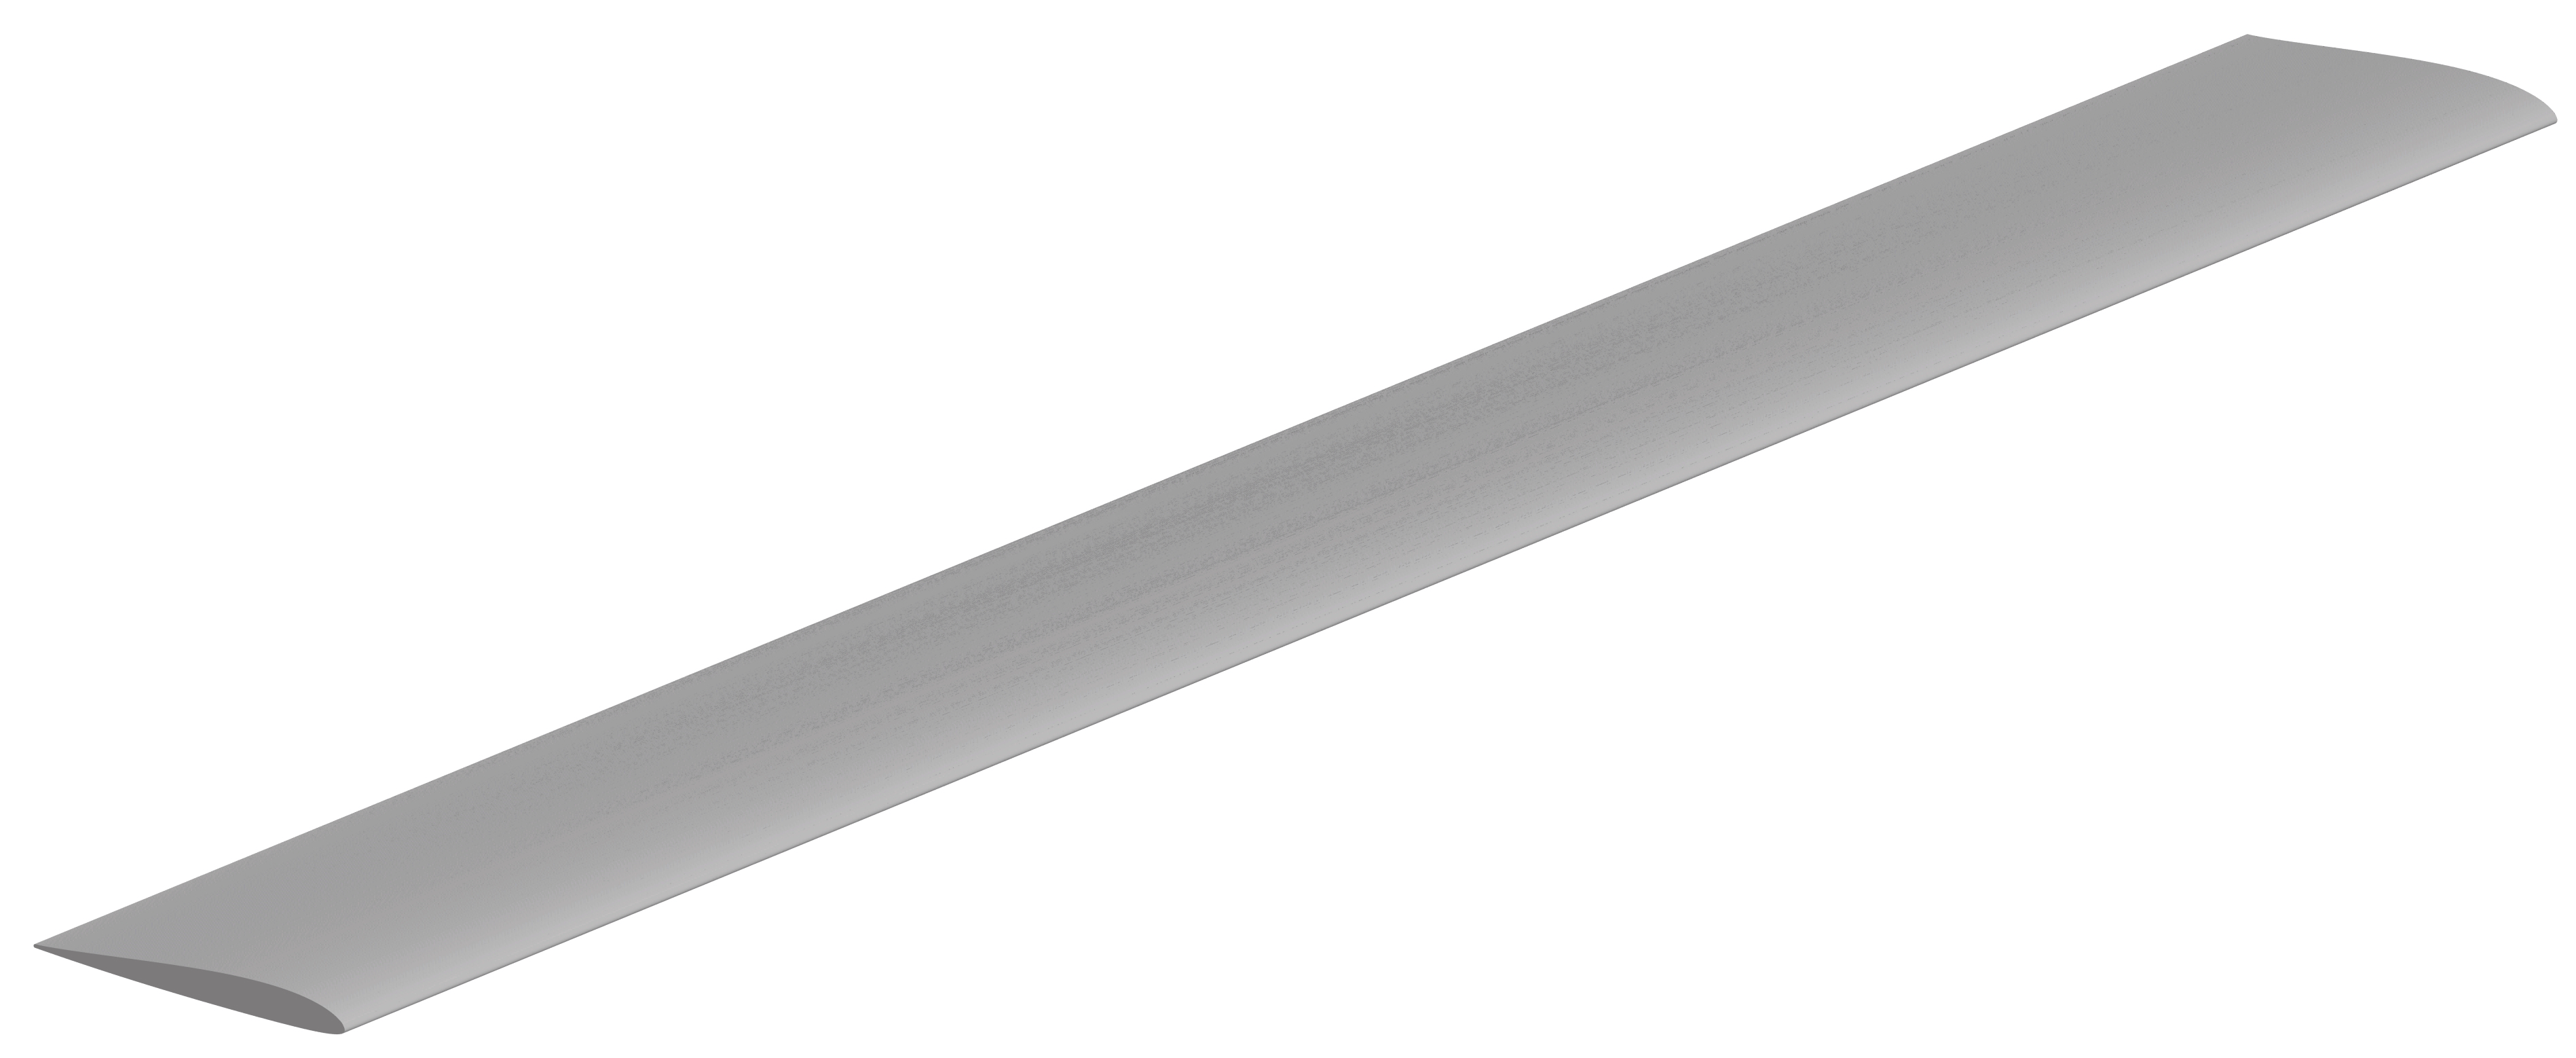
\includegraphics  [ height=6cm] {images/FileImg/rendering.jpg}
\caption{\footnotesize Rendering ala di elevato allungamento con profilo costante PW106. \newline CATIA V5\-6R2017}
\label{fig:catia}
\end{figure}